\documentclass{beamer}
\usetheme[sectionpage=none]{metropolis}

\usepackage{isabelle,isabellesym}
\newcommand*{\term}[1]{{\isaspacing\isastyle \input{#1}}}
\newcommand*{\Term}[1]{{\isaspacing\isastyle #1}}
\newcommand*{\mTerm}[1]{\text{\Term{#1}}}

\usepackage{mathtools}

\DeclarePairedDelimiter\card{\lvert}{\rvert}
\newcommand{\cons}{\mathbin{\#}}

\usepackage[ruled]{algorithm2e}
\resetcounteronoverlays{algocf}


\SetKwInput{Init}{Initialization}
\SetKwInput{Online}{Online Matching}
\SetKwFor{Arrival}{On arrival of}{}{}
\SetKwIF{If}{ElseIf}{Else}{if}{}{else if}{else}{}

\title{Formal Verification of the RANKING algorithm for Online Bipartite Matching}
\author{Christoph Madlener}
\date{22.06.2022}

\begin{document}
\begin{frame}[plain]
  \titlepage
\end{frame}

\section{Introduction}
\begin{frame}
  \frametitle{Online Bipartite Matching (OBM)}
  \begin{columns}
    \begin{column}{.65\textwidth}
      \begin{exampleblock}{Input}
        \begin{itemize}[<+->]
          \item \emph{bipartite} graph $G = (U,V,E)$
          \item \emph{offline} vertices $V$ are known
          \item \emph{online} vertices $U$ reveal edges on arrival
        \end{itemize}
      \end{exampleblock}
    \end{column}
    \begin{column}{.3\textwidth}
      \only<1>{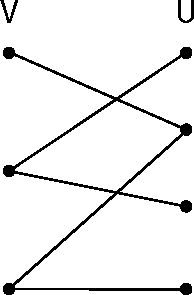
\includegraphics[scale=0.7]{figures/graph_complete}}%
      \only<2-3>{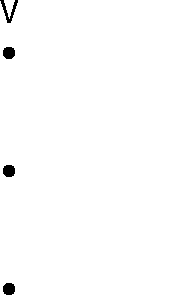
\includegraphics[scale=0.7]{figures/graph_offline_only}}%
      \only<4>{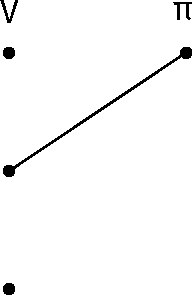
\includegraphics[scale=0.7]{figures/graph_arrival_1}}%
      \only<5>{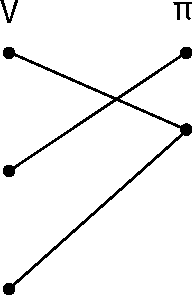
\includegraphics[scale=0.7]{figures/graph_arrival_2}}%
      \only<6>{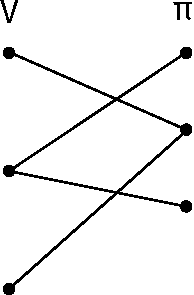
\includegraphics[scale=0.7]{figures/graph_arrival_3}}%
      \only<7>{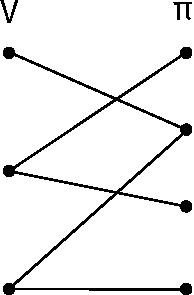
\includegraphics[scale=0.7]{figures/graph_arrival_4}}%
      \only<8-9>{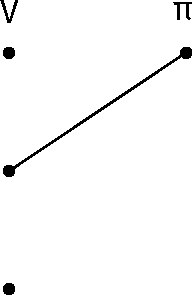
\includegraphics[scale=0.7]{figures/graph_matching_1}}%
      \only<10>{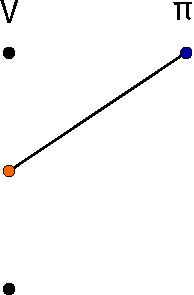
\includegraphics[scale=0.7]{figures/graph_matching_2}}%
      \only<11>{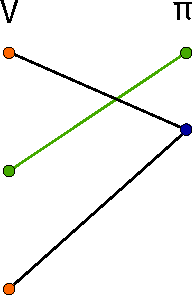
\includegraphics[scale=0.7]{figures/graph_matching_3}}%
      \only<12>{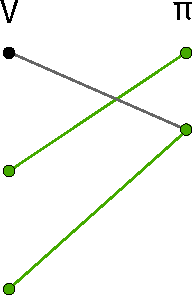
\includegraphics[scale=0.7]{figures/graph_matching_4}}%
      \only<13>{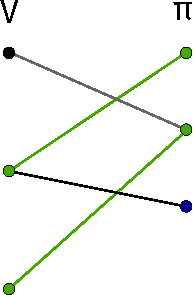
\includegraphics[scale=0.7]{figures/graph_matching_5}}%
      \only<14>{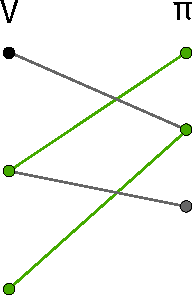
\includegraphics[scale=0.7]{figures/graph_matching_6}}%
      \only<15>{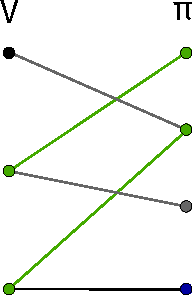
\includegraphics[scale=0.7]{figures/graph_matching_7}}%
      \only<16>{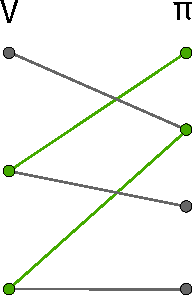
\includegraphics[scale=0.7]{figures/graph_matching_8}}%
    \end{column}
  \end{columns}
  \onslide<8->
  \begin{alertblock}{Task}
    \begin{itemize}
      \item<8-> on arrival of $u \in U$, match to \emph{unmatched} neighbor $v \in V$ (or not)
      \item<9-> maximize size of resulting matching
    \end{itemize}   
  \end{alertblock}
\end{frame}

\begin{frame}
  \frametitle{Competitive Ratio}
  \begin{columns}
    \begin{column}{.65\textwidth}
      \begin{alertblock}{Performance of online algorithm $\mathcal{A}$}
        \begin{itemize}
          \item Compare $\mathcal{A}$ to best offline algorithm
        \end{itemize}
      \end{alertblock}
    \end{column}
    \begin{column}{.3\textwidth}
      \only<1>{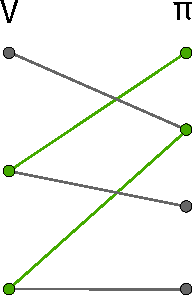
\includegraphics[scale=0.7]{figures/graph_matching_8}}%
      \only<2->{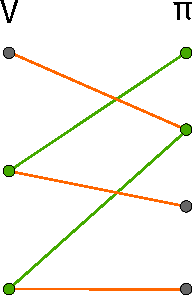
\includegraphics[scale=0.7]{figures/graph_comp_ratio}}
    \end{column}
  \end{columns}
  \onslide<3->
  \begin{block}{Competitive ratio for OBM}
    \only<-3>{\[
      \min_G \min_\pi \frac{\card{\mathcal{A}(G,\pi)}}{\card{M}}
    \]}
    \only<4->{\[
      \min_G \min_\pi \frac{\mathbb{E}\big[\card{\mathcal{A}(G,\pi)}\big]}{\card{M}}
    \]}
    where $M$ is a maximum cardinality matching in $G$.
  \end{block}
\end{frame}

\begin{frame}
  \frametitle{RANKING}
  \onslide<+->
  \begin{itemize}
    \item simple randomized algorithm due to Karp, Vazirani, and Vazirani is optimal~\cite{karp1990}
  \end{itemize}
  \onslide<+->
  \begin{algorithm}[H]
  \small
  \DontPrintSemicolon
  \caption{RANKING}\label{alg:ranking}
  \Init{Choose a random permutation (ranking) $\sigma$ of $V$}
  \Online{}
  \Arrival{$u \in U$}{
    $N(u) \gets \text{set of unmatched neighbors of }u$\\
    \If{$N(u) \neq \emptyset$}{
      match $u$ to the vertex $v \in N(u)$ that minimizes $\sigma(v)$
    }
  }
  \end{algorithm}
  \onslide<+->
  \begin{itemize}
    \item competitive ratio of $1 - \frac{1}{e}$ (best possible)
  \end{itemize}
\end{frame}

\begin{frame}
  \frametitle{Formalization Outline}
  \begin{itemize}[<+->]
    \item formalization follows proof due to Birnbaum \& Mathieu~\cite{birnbaum2008}
    \item three parts
    \begin{enumerate}
      \item \only<3-5>{Combinatorics} \only<6->{\textbf{Combinatorics}}
      \item Probability theory
      \item Competitive ratio in the limit
    \end{enumerate}
  \end{itemize}
\end{frame}

\section{Combinatorics}

\begin{frame}
  \frametitle{Reducing Analysis to Graphs with Perfect Matching}
  \begin{itemize}[<+->]
    \item original paper (and earlier simplifications) assume $G$ has a perfect matching
    \item Birnbaum \& Mathieu state a \alert{\emph{simple structural observation}} which allows to
      generalize to arbitrary graphs:
      
      \vspace{1em}
      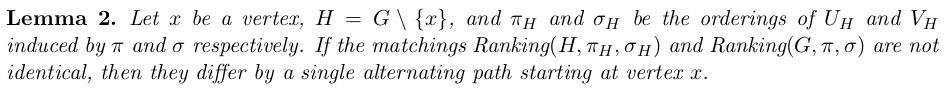
\includegraphics[width=0.9\textwidth]{figures/lemma2}
  \end{itemize}
  \onslide<3->
  Let $G_i$ be the graph resulting from removing $i$ vertices from $G$, which are not in a maximum cardinality matching $M$, and
  $R_i := Ranking(H_i, \pi_{H_i}, \sigma_{H_i})$.
  \onslide<4->
  \[
    \frac{\card{Ranking(G,\pi,\sigma)}}{\card{M}} \geq \frac{{\card{R_1}}}{\card{M}} \geq \dots 
    \geq \frac{{\card{Ranking(G^*, \pi_{G^*}, \sigma_{G^*})}}}{\card{M}}
  \]
\end{frame}

\begin{frame}
  \frametitle{First proof of a \emph{simple structural observation}}
  \begin{columns}
    \begin{column}{.3\textwidth}
      \only<1>{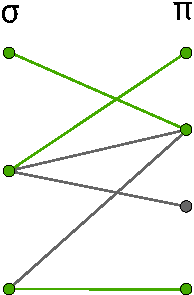
\includegraphics[scale=1]{figures/ranking_before}}%
      \only<2->{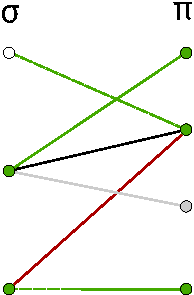
\includegraphics[scale=1]{figures/ranking_after}}
    \end{column}
    \begin{column}{.65\textwidth}
      \onslide<3->
      Let $R := Ranking(G,\pi,\sigma)$ for a fixed graph $G$, arrival order $\pi$, and ranking $\sigma$.
      \begin{alertblock}{Specification of alternating path}
      \begin{align*}
        zig(x) &=
          \begin{cases}
            x \cons zag(y) & \{x,y\} \in R \\
            [x] & x \text{ unmatched}
          \end{cases} \\\\
        zag(y) &=
          \begin{cases}
            y \cons zag(x') & x' \text{ \alert{matched instead}} \\
            [y] & \text{no other match}
          \end{cases}
      \end{align*}
      \end{alertblock}
    \end{column}
  \end{columns}
  \note[itemize]{
    \item \emph{non-recursive} specification of matching on $G$ with arrival order $\pi$,
          and ranking $\sigma$
    \item gives interchangeability of offline and online vertices
    \item symmetry \textrightarrow{} $zig$-$zag$ also works for removing online vertex
    \item full specification of path with mutually recursive functions \emph{zig} and \emph{zag}
    \item Berge's Lemma formalized by Abdulaziz~\cite{abdulaziz2019}
    \item Berge's Lemma not required for Lemma 2, but for consequence
  }
\end{frame}

%\begin{frame}
%  \frametitle{Remaining combinatorics}
%\end{frame}

\section{Randomization}
\begin{frame}
  \frametitle{Randomization}
  \begin{itemize}[<+->]
    \item rephrase everything as \emph{\_ pmf} (probability mass function)
    \item finite probability spaces over permutations \textrightarrow{} lots of sums
  \end{itemize}
  \onslide<+->
  \begin{alertblock}{Switching probability spaces}
    \begin{enumerate}[<+->]
      \item choosing a random permutation \textbf{vs.}
      
      \item choosing a random permutation, a random vertex, and putting that vertex at index $t$
    \end{enumerate}
    \onslide<+->
    For $t = 1$ and $V = \{1,2,3\}$:
    \begin{align*}
      \mathbb{P}_1\Big(\big\{[3,2,1]\big\}\Big) &= \frac{1}{3!} \\
      \mathbb{P}_2\Big(\big\{[3,2,1]\big\}\Big) &= \mathbb{P}_1\Big(\big\{[2,3,1], [3,1,2], [3,2,1]\big\}\Big) 
        \cdot \mathbb{P}_V\big(\{2\}\big) \\
        &= \frac{3}{3!} \cdot \frac{1}{3} = \frac{1}{3!}
    \end{align*}
  \end{alertblock}
\end{frame}

\begin{frame}
  \frametitle{References}
  
  \nocite{github-repo}
  \bibliographystyle{alpha}
  \bibliography{../document/root}
\end{frame}

\end{document}

